\chapter{Another Dimension}

\begin{quote}
Another dimension, another dimension, another dimension, another
dimension, another dimension, another dimension, another dimension,
another dimension, another dimension, another dimension, another
dimension, another dimension!  

\hfill---The Beastie Boys

%\begin{tabular}{rl}
%\textit{Sphere:}     & But where is this land of Four Dimensions? \\
%\textit{I:}          & I know not: but doubtless my Teacher knows. \\
%\textit{Sphere:}     & Not I. There is no such land. The very idea of\\
%                     & it is utterly inconceivable.
%\end{tabular}
%\hfill---E.A.\ Abbott, \textit{Flatland} %p102
\end{quote}

\section{Tessellations}

Go to the internet and look up M.C.\ Escher.\index{Escher, M.C.} He
was an artist. Look at some of his work. When you do your search be
sure to include the word ``tessellation''. OK? Back already? Very
good. Sometimes Escher worked with tessellations. What's a
tessellation? I'm glad you asked:

\begin{dfn}\index{tessellation} A \textbf{tessellation} is a pattern of 
polygons fitted together to cover the entire plane without
overlapping.  
\end{dfn}
While it is impossible to actually cover the entire plane with shapes,
if we give you enough of a tessellation, you should be able to continue
its pattern indefinitely.  Here are pieces of tessellations:
\[
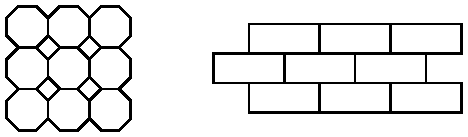
\includegraphics{../graphics/semiRegTess.pdf}
\]
On the left we have a tessellation of a square and an octagon. On the
right we have a ``brick-like'' tessellation.

\begin{dfn}\index{tessellation!regular}\index{regular!tessellation}
A tessellation is called a \textbf{regular tessellation} if it is
composed of copies of a single regular polygon and these polygons meet
vertex to vertex.\index{regular!polygon}
\end{dfn}


\begin{eg} Here are some examples of regular tessellations:
\[
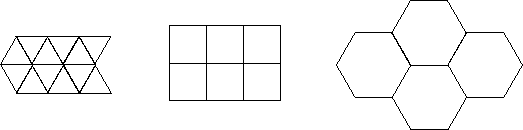
\includegraphics{../graphics/regtess.pdf}
\]
\end{eg}

Johannes Kepler\index{Kepler, Johannes}, who lived from 1571--1630,
was one of the first people to study tessellations. He certainly knew
the next theorem:

\begin{thm} There are only three regular tessellations.
\end{thm}

\begin{ques} Why is the theorem above true?
\end{ques}
\QM

Since one can prove that there are only three regular tessellations,
and we have shown three above, then that is all of them. On the other
hand there are lots of nonregular tessellations. Here are two
different ways to tessellate the plane with a
triangle:\index{tessellation!triangles}
\[
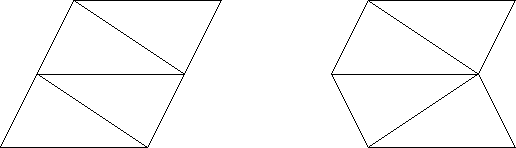
\includegraphics{../graphics/triangletess.pdf}
\]
Here is a way that you can tessellate the plane with any old
quadrilateral:
\[\index{tessellation!any quadrilateral}\index{quadrilateral!tessellation of}
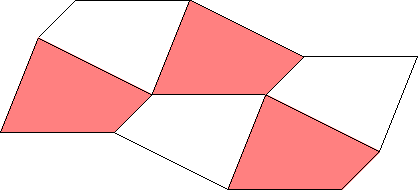
\includegraphics{../graphics/quadtess.pdf}
\]

\subsection{Tessellations and Art}

How does one make art with tessellations? To start, a little
decoration goes a long way. Check this out: Decorate two squares as
such:
\[

\includegraphics{../graphics/lightningsquares.pdf}
\]
Tessellate them randomly in the plane to get this lightning-like picture:
\[
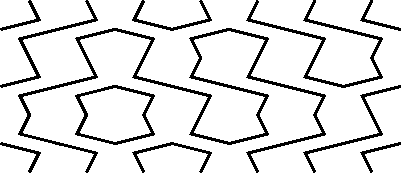
\includegraphics{../graphics/lightningtess.pdf}
\]
\begin{ques} 
What sort of picture do you get if you tessellate these decorated
squares randomly in a plane?
\[
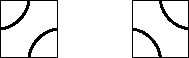
\includegraphics{../graphics/watersquares.pdf}
\]
\end{ques}
\QM

Another way to go is to start with your favorite tessellation:
\[
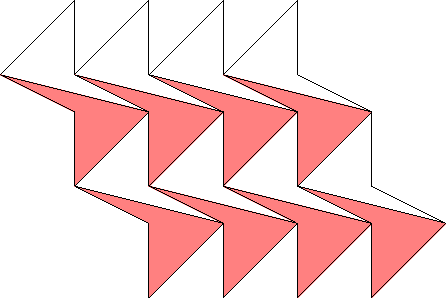
\includegraphics{../graphics/nonconvextess.pdf}
\]
Then you modify it a bunch to get something different:
\[
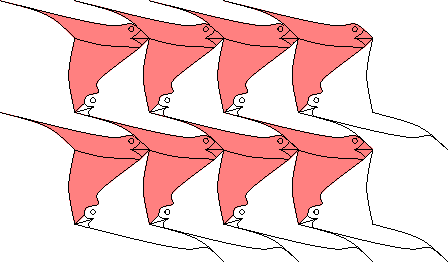
\includegraphics{../graphics/birdstess.pdf}
\]

\begin{ques} What kind of art can you make with tessellations?
\end{ques}
\QM


I'm not a very good artist, but I am a mathematician. So let's use a
tessellation to give a proof! Let me ask you something:

\begin{ques} What is the most famous theorem in mathematics? 
\end{ques}
Probably the Pythagorean Theorem comes to mind. Let's recall the statement of the Pythagorean Theorem:

\begin{thm}[Pythagorean Theorem]\index{Pythagorean Theorem} Given a right triangle, the sum of the squares of the 
lengths of the two legs is equal to the square of the length of 
the hypotenuse.  Symbolically, if $a$ and $b$ represent the 
lengths of the legs and $c$ is the length of the hypotenuse, 
\[
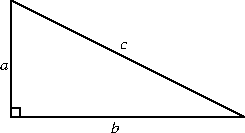
\includegraphics{../graphics/pbppyth.pdf}
\]
then 
\[
a^2 + b^2 = c^2.
\]
\end{thm}


Let's give a proof! Check out this tessellation involving $2$ squares:
\[
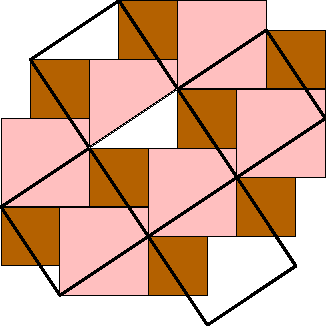
\includegraphics{../graphics/pbppyth2.pdf}
\]
\begin{ques} How does the picture above ``prove'' the Pythagorean Theorem?
\end{ques}
\begin{proof}[Solution]  
The white triangle is our right triangle. The area of the middle
overlaid square is $c^2$, the area of the small dark squares is $a^2$,
and the area of the medium lighter square is $b^2$. Now label all the
``parts'' of the large overlaid square:
\[
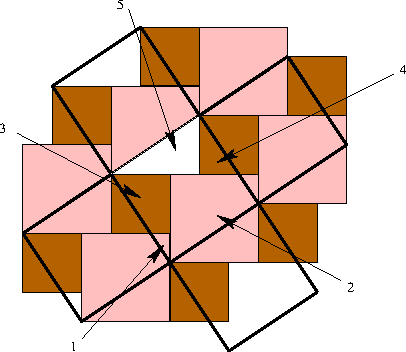
\includegraphics{../graphics/pbppyth2a.pdf}
\]
From the picture we see that
\begin{align*}
a^2 &= \{\text{3 and 4}\}\\
b^2 &= \{\text{1, 2, and 5}\}\\
c^2 &= \{\text{1, 2, 3, 4, and 5}\}
\end{align*}
Hence
\[
c^2 = a^2 + b^2
\]
Since we can always put two squares together in this pattern, this
proof will work for any right triangle.
\end{proof}

\begin{ques} Can you use the above tessellation to give a dissection proof of the Pythagorean Theorem?
\end{ques}
\QM








\newpage

\problems
\begin{enumerate}
\item Show two different ways of tessellating the plane with a given scalene triangle. Label your picture as necessary.
\item Show how to tessellate the plane with a given quadrilateral. Label your picture.
\item Show how to tessellate the plane with a nonregular hexagon. Label your picture.
\item Give an example of a polygon with $9$ sides that tessellates the plane.
\item Give examples of polygons that tessellate and polygons that do
  not tessellate.
\item Give an example of a single triangle that tessellates the plane where
  either $4$ or $8$ angles come together at each vertex.
\item True or False: Explain your conclusions.
\begin{enumerate}
\item There are exactly 5 regular tessellations.
\item Any quadrilateral tessellates the plane.
\item Any triangle will tessellate the plane.
\item If a triangle is used to tessellate the plane, then it is always
  the case that exactly $6$ angles will fit around each vertex.
\item If a polygon has more than 6 sides, then it cannot tessellate the plane.
\end{enumerate}
\item Given a regular tessellation, what is the sum of the angles
  around a given vertex?
\item Given that the regular octagon has $135$ degree angles, explain
  why you cannot give a regular tessellation of the plane with a
  regular octagon.
\item \label{tesstable} Fill in the following table:
\begin{center}
\begin{tabular}{|c || c| c| c|}\hline
 Regular & Does it      &  Measure & If it tessellates, how  \\
 $n$-gon & tessellate?  &  of an angle &  many surround each vertex?  \\
\hline\hline
$3$-gon &  &  &  \\ \hline
$4$-gon &  &  &  \\ \hline
$5$-gon &  &  &  \\ \hline
$6$-gon &  &  &  \\ \hline
$7$-gon &  &  &  \\ \hline
$8$-gon &  &  &  \\ \hline
$9$-gon &  &  &  \\ \hline
$10$-gon &  &  &  \\ \hline
\end{tabular}
\end{center}
Hint: A regular $n$-gon has interior angles of $180(n-2)/n$ degrees. 
\begin{enumerate}
\item What do the shapes that tessellate have in common?
\item Make a graph with the number of sides of an $n$-gon on the
  horizontal axis and the measure of a single angle on the vertical
  axis. Briefly describe the relationship between the number of sides
  of a regular $n$-gon and the measure of one of its angles.
\item What regular polygons \textit{could} a bee use for building
  hives? Give some reasons that bees seem to use hexagons.\index{bees}
\end{enumerate}
\item Considering that the regular $n$-gon has interior angles of
  $180(n-2)/n$ degrees, and using Problem \ref{tesstable} above, prove that
  there are only 3 regular tessellations of the plane.
\item Explain how the following picture ``proves'' the Pythagorean
  Theorem.
\[
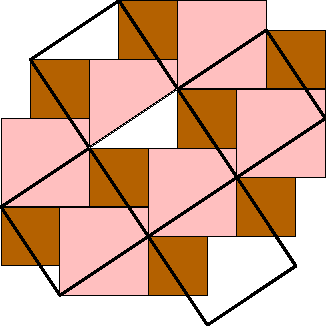
\includegraphics{../graphics/pbppyth2.pdf}
\]
\end{enumerate}

\newpage



\section{Solids}

\subsection{Platonic Solids}\index{Platonic Solids}

Around 2400 years ago, there was a group of mystics---today we might
call it a cult---who called themselves the
\textit{Pythagoreans}.\index{Pythagoreans@The Pythagoreans} Being
mystics, the Pythagoreans had some strange ideas, but on the other
hand they were an enlightened group of people because they believed
that they could better understand the universe around them by studying
mathematics. As part of the Pythagoreans' numerological religion, they
thought that some polyhedra had special powers. The Pythagoreans
associated the following polyhedra to elements of nature:
\begin{center}\index{convex polyhedra!regular}\index{polyhedra!convex regular}
\begin{tabular}{|c|c|}
\hline
Fire: Tetrahedron & Air: Octahedron \\
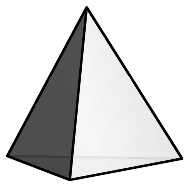
\includegraphics{../graphics/tetrahedron.pdf} 
& 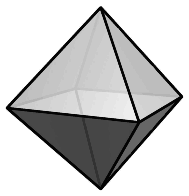
\includegraphics{../graphics/octahedron.pdf} 
\\
\hline 
 Earth: Cube & Water: Icosahedron \\
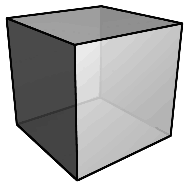
\includegraphics{../graphics/cube.pdf} 
& 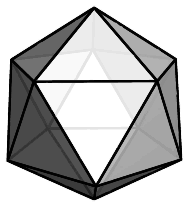
\includegraphics{../graphics/icosahedron.pdf}  
\\
\hline
\end{tabular}
\end{center}
While the idea that these polyhedra are somehow connected to ``arcane
elements of nature'' is complete nonsense, there is actually something
special about the solids above. They are \textit{regular convex
  polyhedra}. Let's dissect those last words:

\begin{dfn}\index{polyhedron} 
A \textbf{polyhedron} is a three dimensional solid that is bounded by
a finite number of polygons.
\end{dfn}

\begin{dfn}\index{convex} 
An object is \textbf{convex} if given any two points inside the object,
the segment connecting those two points is also contained inside the
object.
\end{dfn}

\begin{dfn}\index{regular!polyhedron} 
A polyhedron is \textbf{regular} if all its faces are the same regular
polygon and if the same number of polygons meet at every vertex.
\end{dfn}

Apparently the Pythagoreans discovered the above four regular convex
polyhedra first. Only later did they discover a fifth, the
dodecahedron:
\begin{center}
\begin{tabular}{|c|}
\hline
\AE ther: Dodecahedron\\
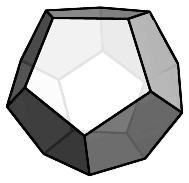
\includegraphics{../graphics/dodecahedron.pdf} 
\\
\hline
\end{tabular}
\end{center}
Since the first four regular convex solids had elements associated to
them, the Pythagoreans reasoned that this fifth solid must also be
associated to an element. However, all the elements were accounted
for. So the Pythagoreans associated the dodecahedron to what we might
call the \index{aether@\ae ther}\ae ther, a mysterious non-earthly
substance.




\begin{ques} 
Consider the \index{triangular dipyramid}\textbf{triangular
  dipyramid}, the solid where two tetrahedrons are joined at a face:
\[
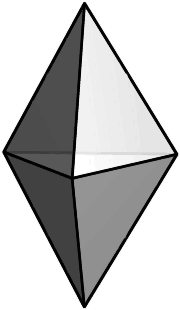
\includegraphics{../graphics/triangulardipyramid.pdf}
\]
Is this a regular convex polyhedron? Explain your reasoning.
\end{ques}
\QM

\begin{ques} Are there regular convex polygons other than the ones shown above?
\end{ques}

We'll give you the answer to this one:

\begin{thm}\label{T:5CP} There are at most five regular convex polyhedra.
\end{thm}

\begin{proof} 
To start, a corner of a three-dimensional object made of polygons must
have at least 3 faces. Now start with the simplest regular polygon, an
equilateral triangle. You can make a corner by placing:
\begin{enumerate}
\item 3 triangles together.
\item 4 triangles together.
\item 5 triangles together.
\end{enumerate}
Each of the above configuration of triangles could give rise to a
regular convex polyhedra.  However, you cannot make a corner out of 6
or more equilateral triangles, as 6 triangles all connected lie flat
on the plane.

Next, we can make a corner with 3 square faces, but we cannot make a
corner with 4 or more square faces as 4 or more squares lie flat on
the plane.

Finally, we can make a corner with 3 faces each shaped like a regular
pentagon, but we cannot make a corner with 4 or more regular
pentagonal faces as they will be forced to overlap.

Could we make a corner with 3 faces each shaped like a regular
hexagon? No, because any number of hexagons will lie flat on the
plane. A similar argument works to show that we cannot make a corner
with 3 faces shaped like a regular $n$-gon where $n>6$, except now
instead of the shapes lying flat on the plane, they overlap.

Thus, we could have at most 5 regular convex polyhedra.
\end{proof}

\begin{ques}
Above we prove that there are at most 5 regular convex polyhedra. How
do we know that these actually exist?
\end{ques}
\QM

The five regular convex polyhedra came to be known as the
\index{Platonic Solids}\textbf{Platonic Solids} over 2000 years ago
when Plato discussed them in his work \textit{Timaeus}. Here is an
empty table of facts about the Platonic Solids---could you be so kind
and fill it in?\index{Platonic Solids}
\begin{center}
{
\renewcommand{\arraystretch}{1.5}
\begin{tabular}{|l|c|c|c|}\hline
Solid & vertices & Edges & Faces\\
\hline\hline
tetrahedron &  &   &   \\ \hline
octahedron &   &  &   \\ \hline
cube &  &   &  \\ \hline
icosahedron &  &  &  \\ \hline
dodecahedron &  &  &  \\ \hline
\end{tabular}}
\end{center}


These solids have haunted men for centuries. People who were trying to
understand the universe wondered why there were
only 5 regular convex polyhedra. Some even thought there was something
\textit{special} about certain numbers.

\begin{ques}
In what ways does the number 5 come up in life that might lead a
person into believing it is a special number? Does this mean that the
number $5$ is more special than any other number?
\end{ques}
\QM

%- In science you usually only hear about the ideas that were right.  BUT
%we only found the right answer by making many many mistakes.
%  In the late 1500s and early 1600s, Johannes Kepler was trying to
%understand the motion of the planets.  He noticed a strange fact.
%
%        There were 6 planets. (known)
%        And there were 5 platonic solids.
%
%Why were there only 6 planets?
%- Kepler believed that they were related to the solids.
%- By nesting the solids inside on another, Kepler believed that they may
%hold the key to the structure of the solar system  at that time the
%universe.
%- Alas, if Kepler had known that there were many more planets and that
%these orbits were defused by gravity

\newpage

\problems
\begin{enumerate}
\item Explain what a \textit{polyhedron} is.
\item Explain what it means for an object to be \textit{convex}.
\item Explain what it means for a polyhedron to be \textit{regular}.
\item State which of the following are convex sets:
\begin{enumerate}
\item A hollow sphere.
\item A half-space.
\item The intersection of two spherical solids.
\item A solid cube.
\item A solid cone.
\item The union of two spherical solids.
\end{enumerate}
In each case, explain your reasoning.
\item Use words and pictures to describe the following objects:
\begin{enumerate}
\item A tetrahedron.
\item An octahedron.
\item A cube.
\item An icosahedron.
\item A dodecahedron.
\item A triangular dipyramid.
\end{enumerate}
\item How is a regular convex polyhedron different from any old convex
  polyhedron?
\item True or False: 
\begin{enumerate}
\item There are only $5$ convex polyhedra.
\item The icosahedron has exactly 12 faces.
\item Every vertex of the tetrahedron touches exactly $3$ faces.
\item The octahedron has exactly $6$ vertices.
\item Every vertex of the dodecahedron touches exactly $3$ faces.
\end{enumerate}
In each case, explain your reasoning.
\item While there are only $5$ regular convex polyhedra, there are
  also nonconvex regular polyhedra. Draw some examples.
\item Draw pictures illustrating the steps of the proof of
  Theorem~\ref{T:5CP}.
\item Where does the proof of Theorem~\ref{T:5CP} use the fact that
  the solids are convex?
\item A \textbf{dual polyhedron}\index{dual!polyhedron} is the
  polyhedron obtained when one connects the centers of all the pairs
  of adjacent faces of a given polyhedron. What are the dual polyhedra
  of the Platonic Solids? Explain your reasoning.
\item How many rotational symmetries does the tetrahedron have?
  Explain your reasoning.
\item How many rotational symmetries does the cube have?
  Explain your reasoning.
\item How many rotational symmetries does the octahedron have?
  Explain your reasoning.
\item How many rotational symmetries does the dodecahedron have?
  Explain your reasoning.
\item How many rotational symmetries does the icosahedron have?
  Explain your reasoning.
\item Consider a cube whose side has a length of 1 unit. Imagine an
  octahedron inside this cube whose vertices are the centers of the
  faces of the cube. How long are the edges of this new octahedron?
\item Consider a tetrahedron whose side has a length of 1
  unit. Imagine another tetrahedron inside the first whose vertices are the
  centers of the faces of the original tetrahedron. How long are the
  edges of this new tetrahedron?
\item Consider a cube whose side has a length of 1 unit. Imagine an
  octahedron around this cube so that the centers of the faces of the
  octahedron are on the vertices of the cube. How long are the edges
  of this new octahedron?
\end{enumerate}



\newpage


\section{Higher Dimensions}


Consider this picture:
\[
\begin{array}{c}
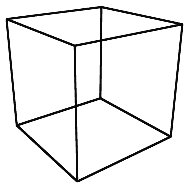
\includegraphics{../graphics/cubeShadow.pdf}\\
\textit{Ceci n'est pas un cube.}
\end{array}
\]
Here, the French got it right. That is not a cube---at best it is what
a \textit{shadow} of a real cube might look like on this sheet of
paper. Since paper is effectively 2-dimensional, it seems
impossible to have an actual cube embedded in this text. The miracle
is that when we look at this shadow of a cube, we know that it
represents a real cube. You may not think this is much of a miracle, but
let's see if I can convince you otherwise. Meet
Sugarbear:\index{Sugarbear}
\[

\includegraphics{../graphics/sugarbear.pdf}
\]
Just as the image at the beginning of this section was a
\textit{picture} of a three-dimensional cube, this is \textbf{not}
actually Sugarbear---rather this is a \textit{picture} of Sugarbear
who is also actually 3-dimensional.


Sugarbear has decided to take a vacation to \textit{Flatland}. The
curious reader should see \cite{abbott} for a history of Flatland.  In
Flatland there are only two directions \textit{left/right} and
\textit{up/down}.  Flatlanders (as they're called) have no concept of
\textit{inward/outward}. As it so happens, you already know someone
from Flatland, Louie Llama!  Here's Louie Llama chilling in front of
his house:
\[
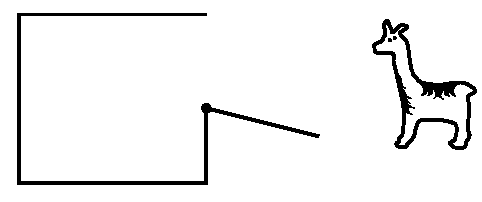
\includegraphics{../graphics/llamaInFlatland.pdf}
\]
Notice, that even when Louie Llama is standing comfortably inside his
house with the door closed, you can still see inside his house! This
is a privilege we receive for living in the third dimension.
\[
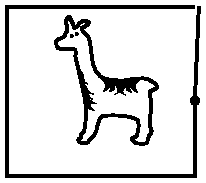
\includegraphics{../graphics/llamaInFlatlandInside.pdf}
\]
On the other hand, Louie Llama cannot see you. From his perspective,
he is surrounded by four walls, and nothing could possibly get inside or
out of his house. So, our favorite llama was quite confused when
Sugarbear greeted him with a jolly ``Hello!'' as she arrived in
Flatland.
\[
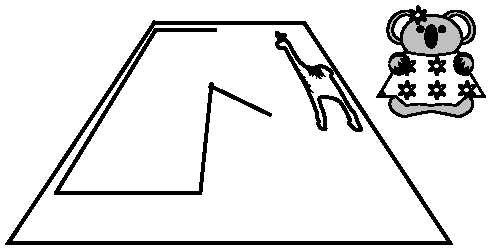
\includegraphics{../graphics/llamaInFlatlandPer.pdf}
\]
Remember, Louie Llama can only see things in the plane that is
Flatland. From Louie Llama's perspective, Sugarbear's ``Hello!''  came
from all around him and even from \textit{inside} himself!  So to help
out the puzzled llama, Sugarbear decided to take the plunge into
Flatland, actually jumping through the plane that Louie Llama lives
in. When she does this, Louie Llama sees something quite strange. Our
llama sees a series of cross-sections of Sugarbear:
\begin{center}
\begin{tabular}{|c|c|c|}
\hline
First & Second & Third\\
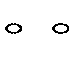
\includegraphics{../graphics/sugarbearCrossSections1.pdf} 
& 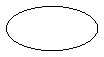
\includegraphics{../graphics/sugarbearCrossSections2.pdf} 
& 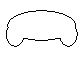
\includegraphics{../graphics/sugarbearCrossSections3.pdf} 
\\
\hline 
Fourth & Fifth & Sixth\\
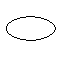
\includegraphics{../graphics/sugarbearCrossSections4.pdf} 
& 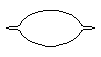
\includegraphics{../graphics/sugarbearCrossSections5.pdf} 
& 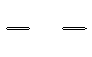
\includegraphics{../graphics/sugarbearCrossSections6.pdf} 
\\
\hline
\end{tabular}
\end{center}

However, each cross-section is very confusing and seems to morph into
the next. This wasn't very helpful for our friend Louie Llama.
\begin{ques}
Can you make sense of what Louie Llama saw?
\end{ques}
\QM 

Sugarbear now says ``Greetings from the third dimension.'' Louie Llama
is quite perplexed---he only knows two dimensions. To help him out,
Sugarbear tries to tell him what a cube is.

\begin{ques}
Can you help Sugarbear describe what a cube is to a two-dimensional
Flatlander? How might Louie Llama react to a real cube?
\end{ques}
\QM

At this point, Sugarbear gets an idea. Why not ``pop'' Louie Llama out
of the plane so that he can see Flatland the way we do?  Being rather
rambunctious for a bear, Sugarbear decides to do this---sending Louie
Llama off into the air floating above Flatland. This is a very strange
experience for Louie Llama.
\[
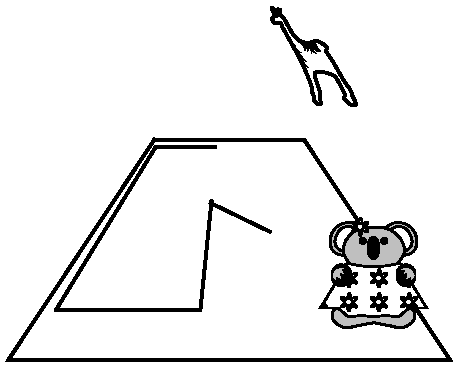
\includegraphics{../graphics/llamaInFlatlandFloat.pdf}
\]
As he floats above Flatland, he can see his world in a way that he had
never seen it before. He can see inside closed buildings and even inside
his friends! Finally, he drifts back down into Flatland. From his
friends' perspective he just ``appeared'' out of nowhere.  When his
friends ask him where he came from, he can only reply, ``up'' but
cannot show them where this is. Louie Llama's worldview has changed
forever.

At the end of her vacation in Flatland, Sugarbear turns to you and
asks you the following question:

\begin{quote}
If Flatlanders had no idea that there could be a third dimension,
who's to say that we are not as blind as they are? Could there be a
fourth dimension?
\end{quote}

\begin{ques}
What would \textit{you} say to Sugarbear? Be careful not to upset her,
her claws are quite sharp.
\end{ques}
\QM

While I honestly don't know if there is a \textit{real} fourth
dimension, we can work by analogy to figure out what it would be like
should it actually exist. We'll start with dimension $0$ and see how
high we can go.

\paragraph{Zero Dimensions} 
A 0-dimensional object is just a point. Draw a point in the box below:
\[

\includegraphics{../graphics/box.pdf}
\]

\paragraph{One Dimension} 
A 1-dimensional object is a segment, what you get from connecting two
points. Draw two points connected by a segment below:
\[

\includegraphics{../graphics/box.pdf}
\]

\paragraph{Two Dimensions} 
There are many different 2-dimensional objects, we'll make a
square. To do this, simply copy the segment you drew above and connect
corresponding end-points. Let's see it in the box below:
\[

\includegraphics{../graphics/box.pdf}
\]

\paragraph{Three Dimensions} 
If you're playing along at home, and I sincerely hope you are, you may
realize that we are going to have a bit of trouble at this point. No
matter: instead of drawing a real cube, we'll draw a ``shadow'' of a
cube. To do this, simply copy the square you drew before, place it
next to the original but offset a little bit. Then connect corresponding
vertices. Let's see your shadow of the cube in the box below:
\[

\includegraphics{../graphics/box.pdf}
\]

\paragraph{Four Dimensions} 
Wow, if we had trouble with three-dimensions, what do we do now? The
answer is simple. We do the same thing we've done before. Simply copy
your shadow of the cube and connect corresponding vertices. Let's see it in the box below:
\[

\includegraphics{../graphics/box.pdf}
\]
Pretty strange, eh? This is called a \textbf{hypercube}\index{hypercube}.

\paragraph{Higher Dimensions} 

We need not stop at dimension four, but as a gesture of friendship---we
will. If we had continued on, we would make a shadow of a
hyperhypercube! That would be pretty mind-blowing.









\paragraph{Some Observations and Thoughts}

Living in a three-dimensional world as we do, it truly seems 
impossible that there could be other dimensions. Yet, it is starting
to seem that perhaps our common sense isn't so sensible. Equipped with
the tool of mathematics, physicists are discovering that our universe
is filled with symmetry. The symmetries we are finding cannot be
explained as the symmetry of any 2-dimensional or 3-dimensional
objects---to explain the observed phenomenon, we need higher
dimensions.



\newpage

\problems
\begin{enumerate}
\item For each of the activities below, explain if they are
  essentially 1-dimensional, 2-dimensional, or 3-dimensional.
\begin{enumerate}
\item Driving a car down the freeway.
\item Riding on a roller coaster.
\item Driving a car in a parking lot.
\item Driving a snowmobile.
\item Flying an airplane.
\item Swimming underwater.
\end{enumerate}
In each case, explain your reasoning.
\item Suppose you stuck your fingers into Flatland. Describe what a
  Flatlander would see.
\item Suppose a 4-dimensional creature stuck its ``fingers'' into our
  three dimensional space. What do you think we would see?
\item Do you know what \textit{bubble tea} is? If not, look it up. It
  is drunk with a large straw that can be used to suck up tapioca
  balls.  Some people love bubble tea, others hate it. If you were a
  tapioca ball in a bubble tea straw, you could only move forward and
  backward, like this:
\[
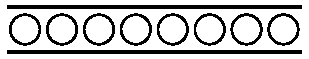
\includegraphics{../graphics/bubble.pdf}
\]
How many dimensions would you view your world in? How many dimensions
would your world actually have? Explain your reasoning.
\item Fill in the following table:
\begin{center}
\begin{tabular}{|c || c| c| c|c|}\hline
 & Vertices & Edges & Faces & Solids \\
\hline\hline
Point &  &  &  & \\ \hline
Segment &  &  &  & \\ \hline
Square &  &  &  & \\ \hline
Cube &  &  &  & \\ \hline
Hypercube &  &  &  & \\ \hline
Hyperhypercube &  &  &  & \\ \hline
\end{tabular}
\end{center}
\item Someone once told me that a simple way to draw a hypercube was
  to draw a regular octagon and then simply make squares on the inside
  of each edge of the octagon. Does this work?  Explain your
  reasoning.
\item We've seen how to draw $n$-dimensional cubes. Explain how to
  draw $n$-dimensional triangles. Draw a triangle, a tetrahedron, and
  a hypertetrahedron. Explain your reasoning.
\item An $n$-sphere is the set of points in $n$ dimensions that are
  all equidistant from a given point. Using this definition, explain
  why:
\begin{enumerate}
\item A $2$-sphere is a circle.
\item A $3$-sphere is a sphere.
\end{enumerate}
In addition, explain what a $1$-sphere would be and do your best to
describe a $4$-sphere.
\item Consider a square whose side has a length of 2 units.
\begin{enumerate}
\item Compute its perimeter and area.
\item Increase the side length of this square by a factor of 3. What
  is the new perimeter and area?
\end{enumerate}
Explain your reasoning. 
\item Consider a cube whose side has a length of 2 units.
\begin{enumerate}
\item Compute its perimeter, area, and volume.
\item Increase the side length of this square by a factor of 3. What
  is the new perimeter, area, and volume?
\end{enumerate}
Explain your reasoning. 
\item Consider a hypercube whose side has a length of 2 units.
\begin{enumerate}
\item Compute its perimeter, area, volume, and hypervolume.
\item Increase the side length of this square by a factor of 3. What
  is the new perimeter, area, volume, and hypervolume?
\end{enumerate}
Explain your reasoning. 
\item If one can only travel along edges, what is the maximum distance
  between two vertices of:
\begin{enumerate}
\item A square whose side has length 1 unit.
\item A cube whose side has length 1 unit.
\item A hypercube whose side has length 1 unit.
\item A hyperhypercube whose side has length 1 unit.
\item An $n$-dimensional cube whose side has length 1 unit.
\end{enumerate}
Explain your reasoning.
\end{enumerate}
